\documentclass[a4paper,11pt]{article}
\input{/home/tof/Documents/Cozy/latex-include/preambule_doc.tex}
\input{/home/tof/Documents/Cozy/latex-include/preambule_commun.tex}
\newcommand{\showprof}{show them}  % comment this line if you don't want to see todo environment
\setlength{\fboxrule}{0.8pt}
\fancyhead[L]{\fbox{\Large{\textbf{Routage 06}}}}
\fancyhead[C]{\textbf{Plus court chemin}}
\newdate{madate}{10}{09}{2020}
%\fancyhead[R]{\displaydate{madate}} %\today
%\fancyhead[R]{Seconde - SNT}
%\fancyhead[R]{Première - NSI}
\fancyhead[R]{Terminale - NSI}
\fancyfoot[L]{\vspace{1mm}Christophe Viroulaud}
\AtEndDocument{\label{lastpage}}
\fancyfoot[C]{\textbf{Page \thepage/\pageref{lastpage}}}
\fancyfoot[R]{\includegraphics[width=2cm,align=t]{/home/tof/Documents/Cozy/latex-include/cc.png}}
\usepackage{tikz}

\begin{document}
\section{Problématique}
Les protocoles de routage (RIP, OSPF) calculent les plus courts chemins entre les routeurs. Les algorithmes utilisés ont été découverts à la fin des années 60 et sont utilisés dans de nombreuses situations.
% RIP déjà utilisé avec ARPANET!
\begin{center}
    \framebox{Comment fonctionnent les algorithmes de plus court chemin?}
\end{center}
\section{Retour des graphes}
\subsection{Graphe orienté}
Un graphe \textbf{orienté} possède les mêmes caractéristiques que celles déjà évoquées pour un graphe non orienté, mais dont les arcs ne peuvent être parcourus que dans un sens. On peut ainsi définir un graphe par \emph{une matrice d'adjacence} ou \emph{un dictionnaire d'adjacence}.
\begin{center}
    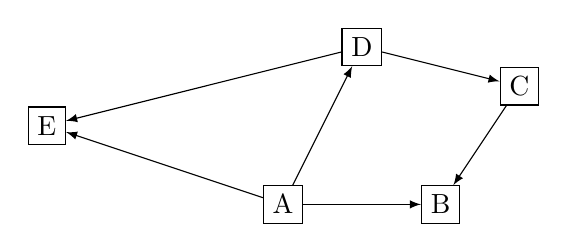
\begin{tikzpicture}
        \node[draw] (A) at (0,0) {A};
        \node[draw] (B) at (2,0) {B};
        \node[draw] (C) at (3,1.5) {C};
        \node[draw] (D) at (1,2) {D};
        \node[draw] (E) at (-3,1) {E};

        \draw[->,>=latex] (A)--(B);
        \draw[->,>=latex] (A)--(E);
        \draw[->,>=latex] (D)--(E);
        \draw[->,>=latex] (A)--(D);
        \draw[->,>=latex] (D)--(C);
        \draw[->,>=latex] (C)--(B);

    \end{tikzpicture}
    \captionof{figure}{graphe orienté}
    \label{oriente}
\end{center}
\begin{aretenir}[]
    Pour chaque nœud on peut définir ses \textbf{prédécesseurs} et ses \textbf{successeurs}.
    \begin{itemize}
        \item Le nœud A ne possède pas de \emph{prédécesseur}.
        \item Le nœud E ne possède pas de \emph{successeur}.
    \end{itemize}
\end{aretenir}
\begin{activite}
    \begin{enumerate}
        \item Établir la matrice d'adjacence du graphe figure \ref{oriente}.
              %la matrice n'est plus symétrique
        \item Établir le dictionnaire d'adjacence du graphe figure \ref{oriente}.
        \item Déterminer un cycle dans le graphe.
    \end{enumerate}
\end{activite}
\subsection{Graphe pondéré}
Les arcs d'un graphe \textbf{pondéré} possèdent une \emph{valeur ou poids}. Cette valeur peut être négative.
\begin{center}
    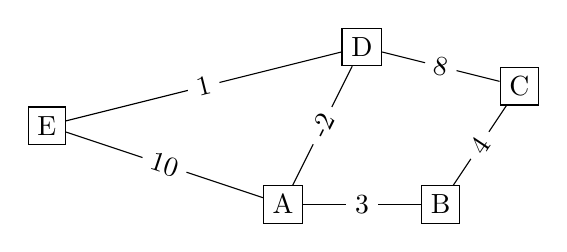
\begin{tikzpicture}
        \node[draw] (A) at (0,0) {A};
        \node[draw] (B) at (2,0) {B};
        \node[draw] (C) at (3,1.5) {C};
        \node[draw] (D) at (1,2) {D};
        \node[draw] (E) at (-3,1) {E};

        \draw (A)--(B) node[sloped, midway, fill=white]{3};
        \draw (A)--(E) node[sloped, midway, fill=white]{10};
        \draw (D)--(E) node[sloped, midway, fill=white]{1};
        \draw (A)--(D) node[sloped, midway, fill=white]{-2};
        \draw (D)--(C) node[sloped, midway, fill=white]{8};
        \draw (C)--(B) node[sloped, midway, fill=white]{4};

    \end{tikzpicture}
    \captionof{figure}{graphe non orienté pondéré}
    \label{pondere}
\end{center}
\begin{activite}
    \begin{enumerate}
        \item Établir la matrice d'adjacence du graphe figure \ref{pondere}.
        \item Établir le dictionnaire d'adjacence du graphe figure \ref{pondere}.
    \end{enumerate}
\end{activite}
\section{Protocole RIP: algorithme de Bellman-Ford}
\subsection{Principe}
Publié entre 1956 et 1958, cet algorithme calcule les plus courts chemins entre un \emph{nœud source} et tous les autres nœuds d'un graphe orienté et pondéré. Le principe est le suivant: 
\begin{center}
    \emph{La distance pour atteindre chaque nœud correspond à la distance pour atteindre son prédécesseur à laquelle on ajoute le poids de l'arête les séparant.}
\end{center}
La démarche est récursive: on applique le même principe au prédécesseur. Enfin un nœud pouvant avoir plusieurs prédécesseurs, on gardera le chemin le plus court.
%approche dynamique bottom-up en pratique
\begin{center}
    \begin{tikzpicture}
        \node[draw] (A) at (0,0) {A};
        \node[draw] (B) at (3,0) {B};
        \node[draw] (C) at (6,0) {C};
        \node[draw] (D) at (9,0) {D};
        \node[draw] (E) at (6,-2) {E};
        \node[draw] (F) at (6,2) {F};

        \draw[->,>=latex] (A)--(B) node[sloped, midway, fill=white]{2};
        \draw[->,>=latex] (B)--(C) node[sloped, midway, fill=white]{6};
        \draw[->,>=latex] (C)--(D) node[sloped, midway, fill=white]{2};
        \draw[->,>=latex] (A)--(F) node[sloped, midway, fill=white]{3};
        \draw[->,>=latex] (B)--(E) node[sloped, midway, fill=white]{4};
        \draw[->,>=latex] (F)--(C) node[sloped, midway, fill=white]{2};
        \draw[->,>=latex] (E)--(C) node[sloped, midway, fill=white]{1};
        \draw[->,>=latex] (E)--(D) node[sloped, midway, fill=white]{5};
        \draw[->,>=latex] (D)--(F) node[sloped, midway, fill=white]{2};

    \end{tikzpicture}
    \captionof{figure}{graphe non orienté pondéré}
    \label{rip}
\end{center}
\begin{aretenir}[Remarque]
Dans le graphe figure \ref{rip} les pondérations représentent un nombre de routeurs traversés pour atteindre le nœud (routeur) suivant.
\end{aretenir}
\subsection{Mise en application}
Chaque routeur exécute l'algorithme pour calculer les plus courts chemins vers chaque autre routeur du réseau. L'algorithme détaillé pour le routeur A est le suivant:
% ligne 2 de l'algo: en effet distance de A à A = 0
\begin{center}
\begin{lstlisting}[language=Bash]
Créer un tableau des distances entre A et les routeurs (A inclus), initialisées à l'infini.
Dans le tableau modifier la distance vers A à 0.

Pour chaque sommet
    Pour chaque arc du graphe
        Si (la distance du routeur) > (la distance de son prédécesseur + poids entre les deux routeurs)
            La distance du routeur est remplacée par cette nouvelle valeur
\end{lstlisting}
\captionof{code}{Algorithme de Bellman Ford}
\label{bf}
\end{center}
Pour le graphe figure \ref{rip}, le tableau est initialisé comme suit:
\begin{center}
    \begin{tabular}{|*{6}{c|}}
        \hline
        A & B & C & D & E & F \\
        \hline
        0 & \infty & \infty & \infty & \infty & \infty \\
        \hline
    \end{tabular}
\end{center}
0n effectue une première itération sur les arcs.\\
La distance calculée pour atteindre B correspond à la distance (du tableau) de son prédécesseur (A) augmentée du poids de l'arc A-B:
$$0+2 = 2 < \infty$$
Le tableau devient:
\begin{center}
    \begin{tabular}{|*{6}{c|}}
        \hline
        A & B & C & D & E & F \\
        \hline
        0 & 2 & \infty & \infty & \infty & \infty \\
        \hline
    \end{tabular}
\end{center}
\begin{activite}
Continuer de dérouler l'algorithme sur le graphe figure \ref{rip}.
\end{activite}
\subsection{Complexité}
La complexité de l'algorithme (code \ref{bf}) dépend:
\begin{itemize}
    \item du nombre de sommets (notée S): on visite chaque sommet (ligne 4);
    \item du nombre d'arcs (notée A): pour chaque sommet on regarde tous les arcs du graphe (ligne 5).
\end{itemize}% extrait de l'algo; ligne 4 = on peut faire une amélioration (normalement on fait pour chaque noeud)
$$O(S.A)$$
\section{OSPF: algorithme de Dijkstra}
\subsection{Principe}
Il a été publié en 1959 par le néerlandais Edsger Dijkstra.
\subsection{Mise en application}
\subsection{Complexité}
\end{document}